\section{Approach}
\label{sec:approach}

\subsection{Environment and System Architecture}
\label{sub:architecture}

Figure~\ref{fig:architecture} illustrates the environment, placement of Zeroties, and the communication between components.
We describe the parts in the Figure by refering to the numbers in the ellipsis.

\begin{figure}[h]
    \centering
    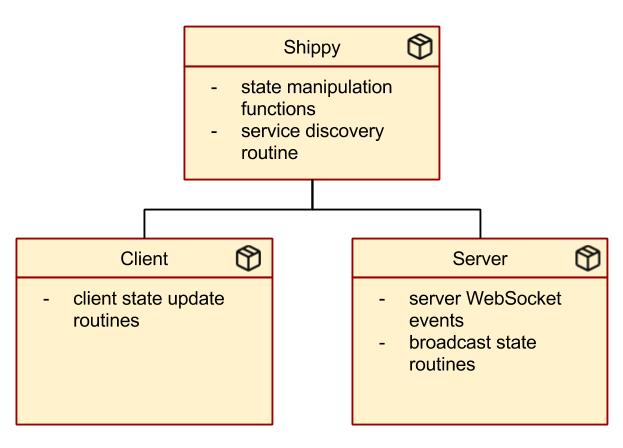
\includegraphics[keepaspectratio,width=6cm]{architecture}
    \caption{System architecture and environment in Zeroties.}
    \label{fig:architecture}
\end{figure}

\begin{enumerate}
\item \textbf{Router}~\footnote{Note that we use the term router somewhat casually in this context. Our notion of router is basically any part in the local network that serves the list of available Zeroconf services, as it can be obtained with DNS-SD. This may involve DHCP, IPv6 Router Advertisement Options or other mechanisms as specified on page 27f of~\cite{cheshire_2013_dnssd}. In other words, we simply call the component that stores the service list obtained from a DNS-SD-capable router.}: we use the protocols provided by Zeroconf (\cite{cheshire_2013_dnssd, cheshire_2013_mdns}) for Zeroties. 
In essence, this means that an authoritative list of currently available Zeroties services (as a subset of all Zeroconf services) can be obtained from the router at any given time.

\item \textbf{Hosts}: there can be an arbitrary number of hosts in our local network. A host can be any device in the network with an instance of Zeroties running (i.e. any device with an OS capable of Zeroconf/DNS-SD protocols).

\item \textbf{Zeroties Daemon}: the instance of Zeroties running on this device. 
This is an OS-level background application maintaining a list of services.
This list is a mirror of the service list obtained from the router by means of the Zeroconf protocols. 
The list of services constitutes the state of the distributed system\footnote{Note that there is a clear line between Successorships and Zeroties: Zeroties does not know about the arbitrarily complex state of Successorships or any other app that builds on Zeroties.}.
We originally intended to integrate this application into browser addons, but were restricted by browser policies.
In particular, there is no possibility to start a web server or publish a Zeroconf service from within a browser addon.
Hence our alternative solution of an OS-level app that communicates with our browser addons through stable bi-directional message channels.

\item \textbf{Browser Addons}: we require browser addons that mediate between web applications and the Zeroties daemon. These addons expose a JavaScript API to apps built on top of Zeroties.
We have implemented addons for Google Chrome and Mozilla Firefox that constitute such a mediator and we have run Successorships apps with these addons (see Section~\ref{sec:evaluation}).
These addons use Zeroties as a publish/subscribe service.
Furthermore, we have built a UI in form of a browser menu button and a popup that shows the currently available list of services.
This UI is refreshed on-the-fly and mirrors the list of services in Zeroties.
Note that the Zeroties daemon itself is not restricted to these addons; they only provide a useful abstraction to web applications running in browsers.
Different applications can utilize the services provided by the Zeroties daemon without these components.

\item \textbf{Publish/Subscribe operations}: applications built on top of Zeroties interact with the Zeroties daemon using the common publish/subscribe operations.
\textit{Publish} is the publishing of a Zeroties service and \textit{subscribe} makes the application receive changes to the list of available Zeroties services. 

\item \textbf{Advertisements and service discovery}: the Zeroties daemon maintains a list of Zeroties services that is obtained from the router.
In a sense, Zeroties acts as a middleware between the router and applications built on top of Zeroties (applications using Successorships as framework being one example). 
Whenever a Zeroties application publishes a service using the Zeroties publish/subscribe API, this will result in the publishing of a service in the network (service advertisement). 
The second part of this communication channel is service discovery.
We describe both service advertisement and service discovery in more detail in Section~\ref{sec:implementation}.
\end{enumerate}


\subsection{Design Decisions and Goals}
\label{sub:design}

Zeroties is based on system models as in the example described in Section~\ref{sec:background_and_motivation}: local ad-hoc network applications. We claim that there is a dedicated set of such applications, for example:
\begin{itemize}
\item a project presentation at a meetup where the audience can connect to the presentation and interact with it.
\item an application for printer control in an office.
\item an application for the heating system of a hotel.
\item multiplayer mode for browser-based games.
\end{itemize}

Such applications have in common a limited number of nodes (generally < 100) and comparably lax requirements for time-to-recovery from system failures: certain downtimes can be tolerated as long as a consistent state is reached eventually.
For example, a running application converging to a consistent state within a time frame of multiple seconds after failures is acceptable.
Our particular goals behind Zeroties are described in the following paragraphs.

\textbf{Publish/subscribe strategy}. 
We reviewed the different publish/subscribe strategies described in~\cite{eugster_2003} and decided to focus on an asynchronous invocation/callback style communication pattern as described in~\cite{eugster_2003}§3.3. 
Asynchrony is essential for the communication between the Zeroties daemon and its applications.
For example, applications built on Zeroties should not be blocked while waiting for the successful advertisement of a service, but rather perform this action in the background while the application remains responsive in the foreground.

\textbf{Consistency guarantees}.
The shared state in Zeroties systems is defined by (1) the list of currently available Zeroties services, and (2) the application-defined state that is shared between hosts in the network.
If an instance is not up-to-date with this state, this can have different consequences. 
First, as long as applications are not notified that a new service has been created, that service remains unavailable.
Second, a service that has failed but remains in the list can result in an error upon connecting to that service. 
Third, if notifications about updates of the application-defined state are delayed between hosts, this can have significant consequences.
However, given our described system model of local ad-hoc network applications, we postulate that it is sufficient for most use cases if hosts converge to a consistent state \textit{eventually} and therefore decided for \textit{optimistic replication}~\cite{saito_2005}.
The paper defines \textit{eventual consistency} as ``a weak guarantee [that] is enough for many optimistic replication applications, but some systems provide stronger guarantees, e.g., that a replica's state is never more than one hour old''.
Due to our requirements for an asynchronous publish/subscribe pattern and our awarenes that, according to the CAP theorem~\cite{gilbert_2012} we cannot achieve both high consistency and availability, our work can be considered as trading consistency in favor of high availability.
Nevertheless, we consider the time frames for reaching consensus in our previous project (> 30 seconds in many cases) as insufficient and we want our new system to do so within a time frame of \textit{5 seconds}.

\textbf{Fault tolerance}:
In the case of Zeroties, fault tolerance is directly connected to consistency guarantees.
Take Successorships as an example for a Zeroties application and assume the scenario of a failing server~\footnote{In the Successorships example, by \textit{server} we refer to the \textit{the currently serving client}. Remember that in our world any client of the web application can become a server.}.
The service that was offered by the failed server will be removed from the list of available Zeroties services and the change will be propagated to Zeroties applications that poll information from the router (see Section~\ref{sub:architecture}).
The application can then decide how to deal with this change.
In the Successorships example, this will involve the selection of a new server (and therefore a new Zeroties service) and other clients connecting to it.
In that sense, the system will have recovered from the failure of the server (and therefore have converged to a consistent state), as soon as (1) the failed service was removed from the list, (2) the newly elected service was added to the list, and (3) all changes propagated to all clients in the system.
Consequently, Zeroties enables its applications to recover from failures in the same time frame as the system reaches consensus.

\textbf{Performance}:
As described earlier, the performance of our previous implementation of Zeroconf based on FlyWeb showed significant bottlenecks and proved insufficient for practical usage.
With Zeroties we had a few concrete goals in mind regarding time frames. 
First, the \textit{publishing of services} and \textit{notifications about new services} from the perspective of a Zeroties application should take \textit{less than 5 seconds}.
\textit{Communication between Zeroties and its applications} should be in the range of \textit{milliseconds}.

\textbf{Reliability}:
Our system should remain highly reliable as long as our DNS-SD communication scheme between Zeroties and the router is robust and the communication channels between Zeroties and its applications are stable.

\textbf{Polling strategy:}
We decided on a polling strategy for obtaining the list of services from the network router using DNS-SD.
The list of available services is updated based on changes detected between the last version of the services list in the Zeroties daemon and the most recently polled services list.
Clearly, this polling strategy will impose traffic on the local network, with all Zeroties hosts polling the router for the services list.
However, we argue that frequent changes in the available services list and the presumed low number of nodes in our system model justifies this approach.
A different strategy which could allow for a larger number of nodes without the potential problem of overloading the router with requests would be to implement this communication with a dedicated Zeroties leader and followers, for example using Paxos~\cite{lamport_2001} or Raft~\cite{ongaro_2014}.
However, this would mostly be a transformation of communication between Zeroties hosts and the router towards host-host communication. 
More importantly, we would waive the advantage of the direct use of the authoritative list of services maintained by the network.
Nevertheless, we are aware that a design with the leader-and-followers approach, despite adding significant complexity, would have advantages as soon as Zeroties networks reach a certain size.


